% Load required classes and packages
\documentclass{mxl-note}
\usepackage{listings}

% Set up document variables
\begin{document}
\title{Mercury2 Preliminary Design}
\author{Jimmy Blanchard}
\docnum{0.1}
\setcounter{secnumdepth}{5}

% Table of Contents
\maketitle
\tableofcontents
\newpage 

\section{Introduction}

Mercury22 is the spiritual successor to the Mercury Ground Station System. It will employ recent advances in web application development and software defined radios to allow satellite operators to easily and efficiently command a network of ground stations across the world.

% Requirements
\section{Requirements}

Mercury2 must be able to perform several core functions. There will be two separate applications: Mercury2 (the web interface), and Iris (ground station task manager). Their core requirements are defined below.

\subsection{Mercury2 Requirements}
Mercury2 will run on a central dedicated server.
\begin{itemize}
	\item Complete user authentication and authorization
		\begin{itemize}
			\item Supports user registrations and account management
			\item Maintains user permissions
		\end{itemize}
	\item Thorough access logs
	\item Satellite operator interface
		\begin{itemize}
			\item Allow satellite operators to automatically schedule passes to best available ground station in specified time window
			\item View signal data for prior passes
		\end{itemize}
	\item Ground station operator interface
		\begin{itemize}
			\item View ground station schedule
			\item Manually download schedules and upload results if not connected to TCP
			\item Manual override to disable automatic scheduling
		\end{itemize}
	\item Complete administration panel
	\item Easy to use interface
	\item SSL encryption and protection from exploits such as XSS cross-site scripting and SQL injection 
\end{itemize}

\subsection{Iris Requirements}
An instance of Iris will run on a computer attached to each ground station radio.
\begin{itemize}
	\item Support multiple radio drivers
	\item Periodically connect to Mercury2 GUI via TCP to download pass schedule and connection settings
	\item Automatically configure radio and transmit/capture data during the time specified by the schedule
	\item Provide satellite operators with a TCP socket to send commands and receive telemetry data
	\item Secure, private key verified transmissions
\end{itemize}

% Architecture Design
\section{Application Architecture}
\begin{figure}[hbtp]
\centering
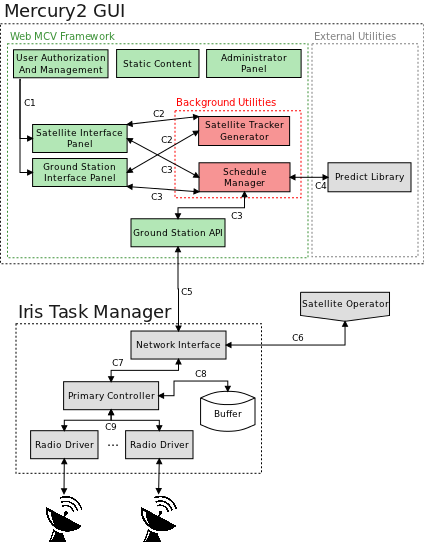
\includegraphics[scale=.65]{Architecture.png}
\caption{Mercury2 and Iris Architecture Overview}
\end{figure}

% Mercury2 GUI Architecture
\subsection{Mercury2 GUI}
The Mercury2 GUI will most likely be a PHP based web MVC framework (e.g. CodeIgniter, CakePHP). An application following this design pattern is broken into models (handle database interactions and various logic tasks), views (the mark up used to display content to the user), and controllers (classes that route users to the appropriate location and join models and views). Figure 1 (above) roughly illustrates the primary controllers that will be used in the application. Each component is explained below. 

\subsubsection{User Authorization and Management}
\begin{description}
	\item [Controller Class]UserController
\end{description}
This section of the website is responsible for managing users and user permissions. It performs several standard user functions, such as account editing, sign-ups, and password recovery. Account creation will be free and open to the public (except, perhaps, in the case of for-profit groups, for which a tiered priced system could be implemented). Once they have made an account, users will be able to submit requests to add satellites (from a list of available TLE's) or ground stations to the website for administrator approval. If approved, the user that submitted the request will gain control of the satellite or ground station's page (described in greater detail in sections 3.1.4 and 3.1.5).

\subsubsection{Static Content}
\begin{description}
	\item [Controller Class]ContentController
\end{description}
This will simply display administrator editable static content to the user such as the FAQs, API documentation, and Terms of Service.

\subsubsection{Administrator Panel}
\begin{description}
	\item [Controller Class]AdminController
\end{description}
The administrator panel will allow administrators to manage Mercury2. In addition to being able to do anything that any other appropriately permissioned user can do (such as viewing signal data, pass schedules, etc.), administrators will be able to:
\begin{itemize}
	\item Manage users
	\item Configure website settings
	\item Create and edit static content
	\item Manually create and edit satellites and ground stations 
	\item Review user requests for new satellites and ground stations
	\item Review application and API statistics
\end{itemize}

\subsubsection{Satellite Interface Panel}
\begin{description}
	\item [Controller Class]SatelliteController
\end{description}
Each satellite that is configured on Mercury2 will have its own set of user accessible pages. Administrators may give any number of users permission to perform some or all actions for any given satellite. In addition, previously authorized users (with the correct permission) may give other users permissions on the page as well. User permissions are managed and verified by the User model and the UserController class described in section 3.1.1. The satellite pages will allow satellite operators to:
\begin{itemize}
	\item View upcoming passes and reserve radio use
	\item View streaming signal data (if the connection permits)
	\item View satellite tracker and AZ/EL chart
	\item View prior pass history
	\item Change basic page design elements such as the logo and color scheme
	\item Upload images and create posts about the satellite
	\item Send an email or text message reporting pass results/status
	\item Give other users permissions on the page
	\item Communicate with ground station operators using private messages
\end{itemize}

\paragraph{Optional Public Page}
In addition to the restricted satellite management page, each satellite will have an optional public page. Some of the page elements described above such as the image gallery and satellite tracker may be added to the public page.

\subsubsection{Ground Station Interface Panel}
\begin{description}
	\item [Controller Class]StationController
\end{description}
Each configured ground station will also receive its own set of pages. The ground station interface will be very similar to the satellite interface in that authorized ground station operators will be able to:
\begin{itemize}
	\item View upcoming and prior passes for the station
	\item View a satellite tracker focused on the ground station
	\item Customize design elements and manage images
	\item View satellite pass history for the station
	\item Add elements to the public page
\end{itemize}
Ground station pages will also allow ground station operators to:
\begin{itemize}
	\item Remove the ground station from the scheduling pool (to take manual control)
	\item Manage queued scheduled passes
	\item Download schedule so that they can manually feed it to ground station (in the case of a ground station with no internet connection)
	\item Manually upload results of a scheduled pass if the ground station was offline at the time
	\item View ground station status and health attributes
	\item Send commands to the ground station
	\item View streamed signal data during passes (if connection permits)
	\item Manage API connection keys (described in section 3.1.6)
	\item Communicate with satellite operators using private messages
\end{itemize}

\subsubsection{Ground Station API}
\begin{description}
	\item [Controller Class]APIController
\end{description}
The APIController will provide API hooks that will allow ground stations to download schedules, report their health and status, and stream signal data to Mercury2 through a UDP socket. The API will consist of a standard REST route scheme and is explained fully in section 3.3.5.

\paragraph{Conflicting Ports}
Because any two satellites may have overlapping pass times (at any combination of ground stations), the UDP sockets opened by the API for the purpose of collecting signal data must be unique and tied to each pass. In addition, they will need to be closed and freed after each pass ends. This could be achieved using a simple CRON job.

\subsubsection{Background Utility: Satellite Tracker Generator}
\begin{description}
	\item [Controller Class]TrackerController
\end{description}
This controller will support an internal API that will provide the necessary framework and configuration settings for instances of the satellite tracker and AZ/EL chart on satellite and ground station pages. Explained more in section 3.3.2.

\subsubsection{Background Utility: Schedule Manager}
\begin{description}
	\item [Controller Class]ScheduleController
\end{description}
The schedule manager will be responsible for managing the requests for ground station use by satellite operators. It will ensure that only one satellite is using any given ground station at a time. All signal and telemetry data collected will be tied to a specified scheduled pass. The schedule management flow is described in below in figure 2.
\begin{figure}[hbtp]
\centering
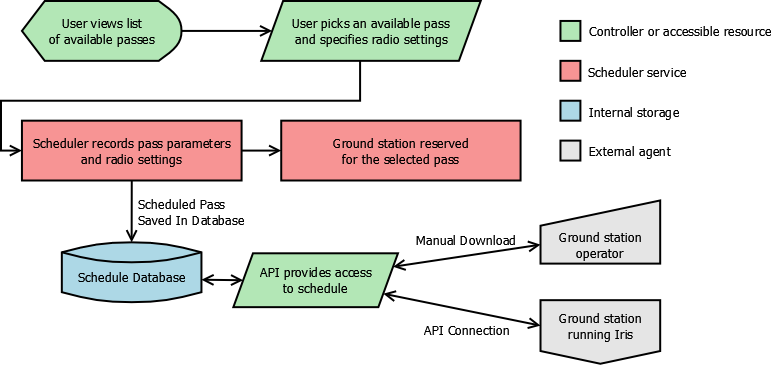
\includegraphics[scale=.4]{SchedulingFlow.png}
\caption{Scheduling process flow}
\end{figure}

\paragraph{Socket Ports}Because the Iris ground station software must provide TCP sockets to enable satellite operators to directly control the satellite and receive telemetry data which may result in overlap between passes (because telemetry data can't be uploaded at the same rate it's received), the scheduler will also determine the ports to use for these sockets. This will allow a scheduled pass to occur while the results of the last pass are still being streamed. This is described more in section 3.2.2.

\subsubsection{External Utility: Predict Library}
\begin{description}
	\item [Type]External API
\end{description} 
Mercury2 will make use of, at least initially, the popular \textit{Predict Library}\footnote{http://www.qsl.net/kd2bd/predict.html} by John Magliacane to calculate pass times. \textit{Predict} provides an API via a network socket that will allow Mercury2 to pass it TLE's and retrieve calculated pass times.

% Iris Task Manager Architecture
\subsection{Iris Task Manager}
The Iris Task Manager program will consist of a relatively simple Python script running on a computer connected to the radio. It will be responsible for downloading the latest schedule, reporting the health of the ground station, connecting to the radio via a set of drivers, streaming signal data, and providing a command/telemetry connection to satellite operators.

\subsubsection{Network Interface}
The network interface class allows Iris to communicate with the Mercury2 GUI. Most communications with Mercury2 will be facilited by connecting to the endpoints provided by the Mercury2 REST API (described in section 3.1.6 and 3.3.5), in addition to a UDP socket for signal data streaming. The network interface class will be responsible for the following:
\begin{itemize}
	\item Downloading the ground station schedule
	\item Reporting the health of the ground station
	\item Streaming signal data
\end{itemize}
In addition, the network interface class must also provide mechanisms to open and close the raw command and telemetry sockets as defined in the schedule.

\paragraph{Network Security}
To ensure secure communication, all interactions between Iris and Mercury2 will be encrypted with a standard SSL encryption scheme. In addition, all communications with Mercury2 will need to be verified using a HMAC-SHA256 private key encryption system which will ensure only the authorized ground stations can access the API.

\subsubsection{Primary Controller}
The primary Iris controller will initialize the program and create the main program loop. This main loop will be responsible for maintaining the state of the ground station and executing scheduled passes. The tasks that it will perform are described below.
\begin{description}
	\item [Fetch Schedules] Periodically (every few minutes) query the network interface class to download the most recent version of the schedule. Also check for offline versions of the schedule if no network connection is available.
	\item [Report Status] Every request for a schedule update will also include information about the health and status of the ground station. For example, the currently executing task and radio parameters may be included. This information will be reported on the ground station and satellite operator pages in the GUI. This mechanism is described in 3.3.5.
	\item [Execute Scheduled Passes] Once a scheduled pass starts, Iris will:
		\begin{itemize}
			\item Attempt to configure the radio via the selected radio driver using the connection settings defined by the schedule
			\item Update the radio status to reflect the connection
			\item Open two sockets to allow satellite operators to submit commands to the satellite and receive telemetry from the pass (ports determined by scheduler to prevent conflict)
			\item Create a thread to maintain the connection during the pass (correct doppler, etc.)
			\item Create a thread to store raw telemetry data into a buffer and feed it to the satellite operator via the telemetry socket
			\item Create a thread to stream signal data back to the GUI by invoking the network interface class
		\end{itemize}
	\item [Complete Scheduled Passes] Once a pass has finished (determined by the schedule calculated by the Predict Library in the GUI), Iris will:
		\begin{itemize}
			\item Update the radio status
			\item Destroy connection maintenance thread 
			\item Destroy signal data stream thread
			\item Check if all telemetry data has been transmitted to the satellite operator. If it has, destroy the thread. Otherwise keep the thread until it streams all of the telemetry data.
		\end{itemize}
\end{description}

\paragraph{Telemetry Persistence}
All of the telemetry data collected will be stored for a certain period, in case there was an error transmitting or receiving it the first time. This will also allow operators running ground stations without internet access the ability to manually retrieve the telemetry from a pass and send it to satellite operators.

\subsubsection{Radio Drivers}
Each type of radio connected will need its own driver class. These classes will be standardized and must provide a mechanism to update the radio settings and gain access to the radio's command and telemetry streams.

\subsection{Connection Details}
The connections shown in figure 1 (labeled C\#) are the primary data routes for the Mercury2/Iris system. They are explained in detail below.

\subsubsection{C1 - User Authorization}
\begin{description}
	\item [Connection Type] Database Model Interaction
\end{description}
When a user requests a satellite or ground station page in their browser, their permissions will be retrieved from the database to determine what control, if any, they should have over the page. Users can be given an arbitrary amount of control over any satellite or ground station by either website administrators or existing users on the ground station/satellite page with the appropriate permissions (i.e. the ability to add new team members).

\subsubsection{C2 - Satellite Tracker Tool}
\begin{description}
	\item [Connection Type] Database Model Interaction
\end{description}
When a satellite or ground station page contains an instance of a satellite tracker, it will use the satellite tracker generator (section 3.1.7) to generate the appropriate configuration for that tracker (e.g. available satellites, ground stations, visual options, etc.). By seperating the tracker configuration generation from the satellite and ground station controllers, it is much more modular and can be included in any configuration on any arbitrary page.

\subsubsection{C3 - Schedule Manager}
\begin{description}
	\item [Connection Type] Database Model Interaction
\end{description}
These connections will allow any page on Mercury2 (particularly the satellite and ground station control panels) to view a subset of the pass schedule. For example, when a user loads a satellite interface page the schedule manager will be queried, through this connection, for the relevant pass schedule. This connection will also allow authorized users to add passes to the schedule or cancel upcoming passes.

\paragraph{API Use}The Mercury2 API will connect to the schedule manager using the same paths and access methods as any other page to retrieve the needed schedule. The only difference is how it will be presented to the end user (e.g. human-readable table vs machine readable API format).

\subsubsection{C4 - Predict Library API}
\begin{description}
	\item [Connection Type] External API Connection
\end{description}
Mercury2 will use the \textit{Predict Library} (section 3.1.9) to calculate the times of upcoming passes. \textit{Predict} is a C application that runs independent of the Mercury2 MVC framework server application. \textit{Predict} provides a TCP socket based API that will allow the Mercury2 schedule manager to load current TLE's and retrieve upcoming passes.

\subsubsection{C5 - Primary Ground Station API}
\begin{description}
	\item [Connection Type] External API Connection
\end{description}
This API will be used by any configured Iris ground station to connect to Mercury2. It will allow ground stations to retrieve the most recent version of its schedule, report its health and status, and stream signal data back to Mercury2. This API will be split into two seperate sections. The first will be a standard HTTP REST API with the following paths and functionality.
\begin{description}
	\item [/api/schedule/:station-name.format] The ground station will POST to this path with its current health and status. The Mercury2 API will respond with a .format (either JSON or XML) encoded string containing the ground station's schedule and radio connection settings for each scheduled event. It will also transmit a checksum to allow the ground station to verify the integrity of the transmission.
\end{description}
In addition, the API will also provide a UDP socket (with a port unique to each pass scheduled) that will allow the ground station to stream back its signal data (signal strength, etc.) to the Mercury2 GUI.

\paragraph{API Security}
API connection security will consist of standard SSL encryption to protect against middle-man attacks and HMAC-SHA256 private key encryption to prevent unauthorized access. Ground station operators will be able to generate and retrieve API keys from the ground station interface page.

\subsubsection{C6 - Satellite Operator Connections}
\begin{description}
	\item [Connection Type] External Socket Connection
\end{description}
When a pass starts, the ground station will open two sockets for use by the satellite operators. One for transmitting commands to the satellite, and one for receiving telemetry data. These sockets will be opened on the ports specified in the schedule (which will be reported to satellite operators when they schedule a pass). After a pass ends, these sockets will be closed.

\subsubsection{C7 - Primary Controller and Network Interface Interaction}
\begin{description}
	\item [Connection Type] Internal Connection
\end{description}
The primary controller (section 3.2.2) will interact with the network interface class to receive schedule data, transmit the ground station health, and provide raw socket access to the radio for satellite operators.

\subsubsection{C8 - Telemetry Buffer}
\begin{description}
	\item [Connection Type] Internal Connection
\end{description}
The primary controller will record all received telemetry and beacon data into an internal buffer (most likely just a file dump). This data will be associated with a scheduled pass and timestamp. It will also be streamed through the telemetry socket to the satellite operator as it is received from the satellite. Because telemetry data is often very large per pass (on the order of gigabytes), it will be rotated every few days. This allows ground station operators to retrieve a copy of the data if requested by the satellite operator (in the case of a transmission or receive failure during the initial pass). 

\subsubsection{C9 - Radio Driver Interface}
\begin{description}
	\item [Connection Type] Internal Connection
\end{description}
The primary controller will connect to each radio driver using a standard class interface. This will provide the mechanism to allow the ground station to configure the radio settings, as defined by the pass schedule. It must also be able to provide a socket to the radio command and telemetry feeds. The specifics of this interface will be defined at a later time.

\end{document}
